\section{Algunos invariantes.}\label{seccion5}
Suponga que cierto día ha ido a trabajar con su portátil fuera de casa y se lo ha dejado olvidado. Cuando te das cuenta, vuelves a buscarlo pero ya no está. Pasan unos días y un amigo te comenta que se ha encontrado un portátil con $x$ número de puertos, procesador $y$ y modelo $z$.\\

Es claro que si alguna de esas características no fuese la de tu portátil, tendrías claro que no es el tuyo. Pero resulta que tu portátil tiene exactamente las mismas características. Piensas que tal vez sea tu portátil pero no tienes garantía de que realmente lo sea. \\

Algo similar, aplicado a nudos, es lo que vamos a tratar de ver en esta sección. ¿Dadas dos proyecciones, podremos decir que representan al mismo nudo? Vamos a tratar de estudiar ciertos invariantes sobre los nudos. Al igual que ocurría con el caso del portátil, si dos proyecciones tienen valores de un invariante distintos podremos decir que no representan al mismo nudo. Sin embargo, si ambos tienen valores de un invariante iguales no podremos saber si se trata del mismo nudo. Tendremos que estudiar otros invariantes de nudos. \\

¿Y si estudiamos una gran cantidad de invariantes de dos proyecciones y siempre toman los mismos valores?¿Podremos garantizar que son equivalentes? La respuesta es clara, no. Tendremos que analizar en mayor detalle las proyecciones, pero puede ser que no lleguemos a obtener un conclusión definitiva. \\


Por tanto, el estudio de invariantes de los nudos nos va a permitir saber si dos nudos pueden ser (destacamos, que no quiere decir que lo sean) o no son equivalentes.\\


Antes de ver algunos de los invariantes de nudos más conocidos y útiles vamos a dar una definición formal de lo que se conoce como un invariante:\\

\underline{\textbf{Definición:}} \\
Un \textbf{invariante} de un nudo (o de un enlace) es una propiedad que no cambia cuando el nudo sufre deformaciones en el espacio. \\



\begin{center}
	\subsection{Número de componentes:}
\end{center}
Es uno de los invariantes de enlaces más sencillos que nos podemos encontrar y que ya hemos comentado ligeramente en las secciones anteriores.\\

Cada componente de un enlace es una curva disjunta del mismo. En la Figura \ref{inv1} vemos un enlace con dos componentes. 
\begin{figure}[h!]
	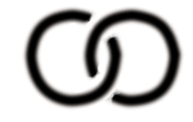
\includegraphics[width=2.7cm]{inudos/enlace.png}
	\centering
	\caption{Enlace con dos componentes.}
	\label{inv1} 
\end{figure}

Al aplicarle a un enlace cualquier transformación no se le puede añadir ni eliminar ninguna componente. De modo que este invariante no nos va a permitir comparar nudos, pues todo nudo tiene una sola componente. \\

\bigskip
\begin{center}
	\subsection{Crossing number:}
\end{center}
Sea un nudo K. Su \textbf{crossing number} es el menor número de cruces que se encuentra en cualquier proyección del nudo. Se denota como $c(K)$. \\

Esto nos lleva a deducir que el nudo K tendrá como mínimo c(K) cruces por muchas transformaciones que se apliquen a sus proyecciones.\\

Aunque es un invariante sencillo de visualizar, no es fácil de obtener: puede ser que al estudiar muchas proyecciones de un nudo pensemos que su número de cruces es $n$, sin embargo pueden existir otras proyecciones del nudo que no conocemos con menor número de cruces. Por este motivo, no vamos a trabajar posteriormente con este invariante.\\

Para dejarlo más claro vamos a ver un ejemplo.\\
Consideramos la proyección de la primera figura \ref{cross1}. Podemos pensar que el número de cruces del nudo sería 4 (ver los 4 cruces de la figura a). Sin embargo, esta proyección es equivalente a la proyección que vamos en la figura b, que tiene como número de cruces el valor 3. Por tanto, el número de cruces del nudo, que es el nudo trébol, es 3. 
\begin{figure}[h!]
	\centering
	\subfigure[4 cruces]{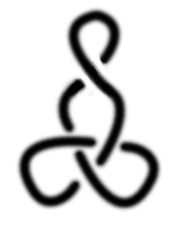
\includegraphics[width=3.4cm]{inudos/3fseg.png}}
	\subfigure[3 cruces]{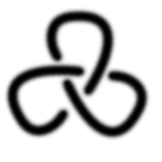
\includegraphics[width=3.4cm]{inudos/3f.png}}
	\caption{Crossing number del nudo trébol.}
	\label{cross1} 
\end{figure}  


\begin{center}
	\subsection{Tricolorabilidad:}
\end{center}
Para definir este invariante de enlaces, tenemos que conocer unos conceptos previos:\\
Entendemos por undercrossing y overcrossing a un recorrido en el cruce de la proyección de un nudo que nos lleva por encima o por debajo en el cruce. \\

Veamos la imagen \ref{tric1} donde queda representado:\\
\begin{figure}[h!]
	\centering
	
\includegraphics[width=7cm]{inudos/cruce.png}
	\caption{Tipo de cruce.}
	\label{tric1} 
\end{figure}

\underline{\textbf{Definición:}}\\
Una\textbf{ hebra }de una proyección de un enlace es una región de cuerda del enlace que va desde un undercrossing a otro undercrossing atravesando sólo overcrossings.\\ 

\underline{\textbf{Definición:}}\\
Una proyección de un enlace es tricolorable si cada una de las hebras de la proyección puede ser coloreada con uno de tres colores diferentes de modo que en cada cruce o los 3 colores se junten o se junte un sólo color. En este caso diremos que el enlace es \textbf{tricolorable}. 

\begin{teo}
	La tricolorabilidad se perserva mediante movimientos de Reidemeister.
	\begin{proof}
		Supongamos que partimos de una proyección de un nudo que es tricolorable y vamos a aplicarle los movimientos de Reidemeister. Tendremos que ver que la proyección final es tricolorable. Podemos centrarnos en la zona de la proyección a la que se le aplica el movimiento. Veamos qué ocurre al aplicar cada movimiento:\\
		
		\underline{R1:}
		En este caso sólo se puede dar que tengamos un sólo color. Al aplicar el movimiento R1 seguiremos utilizando ese mismo color, de modo que la proyección modificada seguirá siendo tricolorable. 
		\begin{figure}[h!]
			\centering
			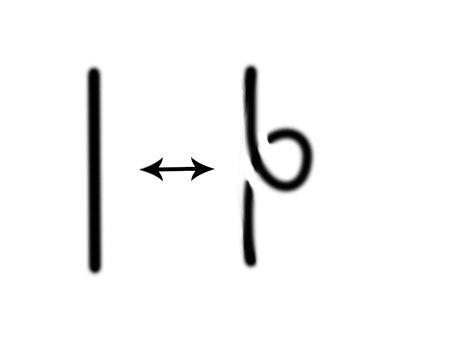
\includegraphics[width=5.5cm]{inudos/movi1.png}
			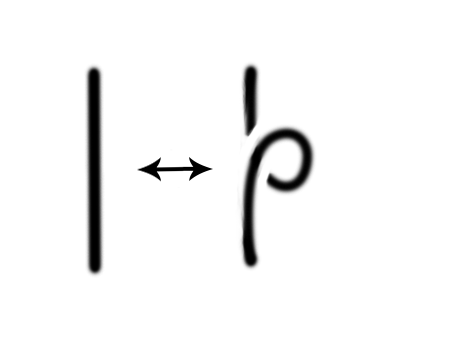
\includegraphics[width=5.5cm]{inudos/movi2.png}
			\caption{Demo R1}
			\label{demotri1} 
		\end{figure}
		
		\underline{R2:}
		Supongamos que el coloreado inicial se ha realizado con un sólo color. Al igual que con el movimiento R1, no tendríamos ninguna dificultad pues al aplicar el movimiento R2 seguiremos coloreando con el mismo color y la proyección seguirá siguiendo tricolorable. \\
		\begin{figure}[h!]
			\centering
			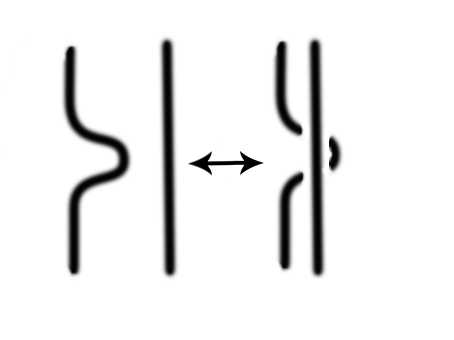
\includegraphics[width=5.5cm]{inudos/movi3.png}
			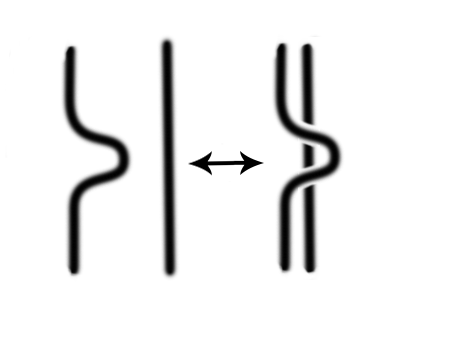
\includegraphics[width=5.5cm]{inudos/movi4.png}
			\caption{Demo R2}
			\label{demotri2} 
		\end{figure}
		
		Ahora tenemos otra segunda opción de coloreado en la proyección inicial y es que en ambos cruces posibles usemos los 3 colores posibles. Se puede ver en la figura \ref{demotri3}. Se observa que la proyección sigue siendo tricolorable. 
		\begin{figure}[h!]
			\centering
			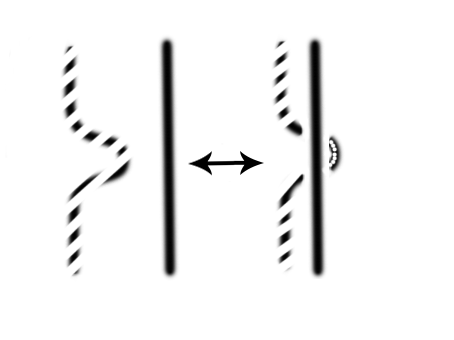
\includegraphics[width=8.3cm]{inudos/movi3tri.png}
			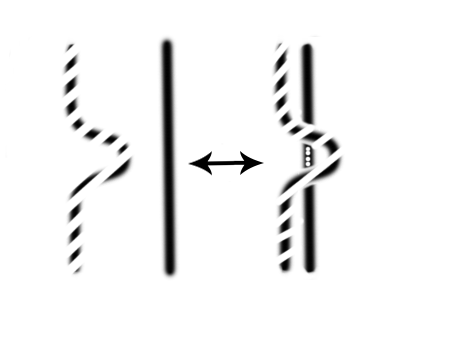
\includegraphics[width=8.3cm]{inudos/movi4tri.png}
			\caption{Demo R2}
			\label{demotri3} 
		\end{figure}
		
		\underline{R3:}
		Este movimiento tiene más complejidad pues tenemos 3 cruces posibles. Analizamos todos los casos posibles y vemos que nos podemos reducir a cinco situaciones. Veamos en la figura \ref{demotri4} cómo sería el cambio de color en cada caso para confirmar que las proyecciones resultantes al aplicar el movimiento siguen siendo tricolorables.
		\begin{figure}[h!]
			\centering
			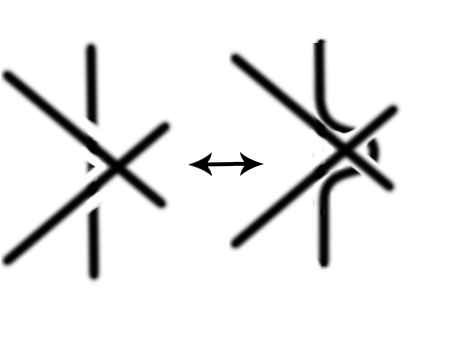
\includegraphics[width=8cm]{inudos/movi5.png}
			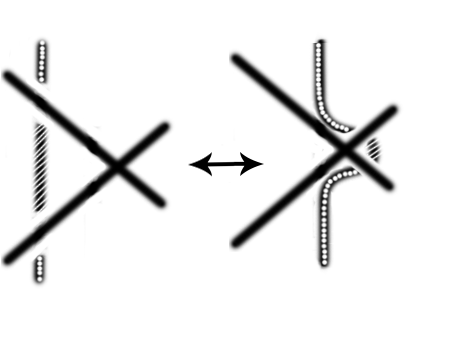
\includegraphics[width=8cm]{inudos/movi5tri1.png}
			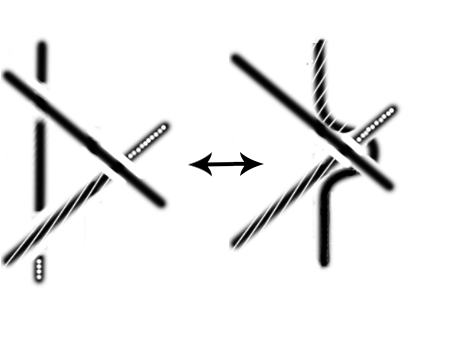
\includegraphics[width=8cm]{inudos/movi5tri2.png}
			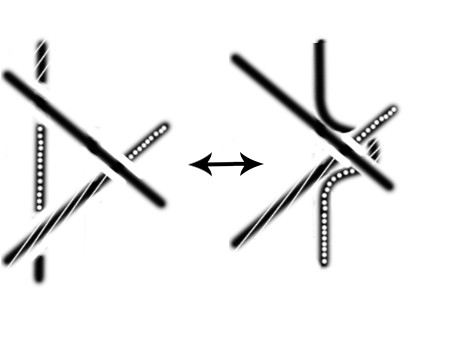
\includegraphics[width=8cm]{inudos/movi5tri3.png}
			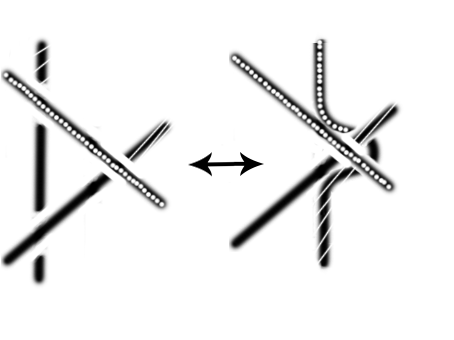
\includegraphics[width=8cm]{inudos/movi5tri4.png}
			\caption{Demo R3}
			\label{demotri4} 
		\end{figure}
		
		Concluimos que si tenemos una proyección tricolorable y aplicamos los movimientos de Reidemeister, la proyección resultante sigue siendo tricolorable. \\
		Si la proyección de partida no fuese tricolorable, la proyección resultante tampoco podría ser tricolorable: supongamos que la proyección resultante es tricolorable, por el razonamiento que hemos seguido anteriormente, tendríamos que tener que la proyección inicial sería tricolorable llegando a contradicción. 
		
	\end{proof}
\end{teo}


Haciendo uso de este invariante podemos demostrar que el nudo trivial y el nudo trébol no son equivalentes, es decir, son topológicamente distintos. Esto se debe a que el nudo trébol es tricolorable pero el nudo trivial no lo es. Podemos verlo en la imagen \ref{Tric2}.\\
\begin{figure}[h!]
	\centering
	\subfigure[No tricolorable]{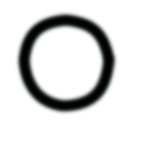
\includegraphics[width=4cm]{inudos/1.jpg}}
	\subfigure[Tricolorable]{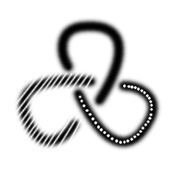
\includegraphics[width=4cm]{inudos/3ftri.png}}
	\caption{Dos nudos no equivalentes.}
	\label{Tric2} 
\end{figure} 


Este hecho confirma que existe al menos un nudo distinto del nudo trivial. Es más, todo nudo que sea tricolorable será distinto del nudo trivial.\\

Sin embargo, este invariante no es muy potente en el sentido de que sólo clasifica los enlaces en tricolorables y no tricolorables y sólo podremos afirmar que dos proyecciones representan a diferentes nudos si una de ellas es tricolorable y la otra no lo es.   


\bigskip
\begin{center}
	\subsection{Unknotting number:}\label{subunk}
\end{center}
Supongamos que tenemos la proyección de un nudo no trivial. Modificar la proyección para que un undercrossing pase a ser un overcrossing, o viceversa, no es un movimiento válido pues estamos intersecando la cuerda. Sin embargo, es un movimiento interesante ya que nos llevará al nudo trivial. \\

\underline{\textbf{Definición:}}
Se define el \textbf{número de desanudamiento} de un nudo como el menor número de cambios en los cruces necesarios para desanudarlo, es decir, para llegar al nudo trivial. Se denota como $u(K)$. \\

Es claro que en un número finito de pasos conseguiremos obtener el número de desanudamiento: Recorremos el nudo con cierta orientación y al llegar a un cruce, si no hemos pasado anteriormente por él y es un undercrossing, lo convertimos en overcrossing. \\ 

Podemos ver, en la figura \ref{unk1}, que el número uno es el número de desanudamiento para el nudo trébol. El punto de partida lo indicamos con un punto grueso.
\begin{figure}[h!]
	\centering
	\subfigure[Nudo de partida]{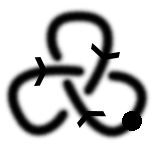
\includegraphics[width=3.4cm]{inudos/3fcon1start.png}}
	\subfigure[Nudo modificado]{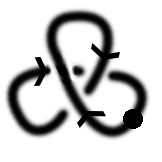
\includegraphics[width=3.4cm]{inudos/3fcon1negstart.png}}
	\caption{Unknotting number trébol.}
	\label{unk1} 
\end{figure}

\bigskip
\begin{center}
	\item \subsection{Polinomio de Alexander:}\label{alenudos}
\end{center}
Anteriormente hemos visto algunos invariantes geométricos y numéricos que nos pueden ayudar en la tarea de comprobar si dos proyecciones representan al mismo nudo. Ahora vamos a ver un invariante polinómico que estudiaremos con más detalle pues será uno de los puntos fuertes que implementaremos para resolver, en parte, la cuestión. \\

Se trata de un polinomio, con variable $t$, para nudos orientados. En 1969, se probó que dicho polinomio puede calcularse computacionalmente haciendo uso de dos reglas:
\begin{itemize}
	\item \underline{Regla 1:} \\
	El polinomio de Alexander del nudo trivial es el polinimio trivial equivalente a 1. Esta regla se representa como $\vartriangle$($\bigcirc$)= 1
\end{itemize}

Para poder exponer la segunda regla tenemos que conocer antes las siguientes ideas. \\
Consideramos el enlace orientado de partida. Si nos centramos en uno de sus cruces, podemos crear tres nuevos enlaces orientados exactamente iguales al de partida variando únicamente en este cruce seleccionado. A cada uno de estos nuevos enlaces le establecemos uno de estos nuevos cruces:
\begin{enumerate}
	\item $L_{+}$: El cruce seleccionado se establece como positivo.
	\item $L_{-}$: El cruce seleccionado se establece como negativo.
	\item $L_{0}$: El cruce seleccionado se elimina.
\end{enumerate}
Podemos ver estos nuevos cruces en la figura \ref{alex1}.\\

\begin{figure}[h!]
	\centering
	\subfigure[$ L_{+} $]{
\includegraphics[width=4cm]{inudos/pro1.png}}
	\subfigure[$ L_{-} $]{
\includegraphics[width=4cm]{inudos/pro2.png}}
	\subfigure[$ L_{0} $]{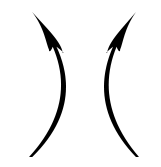
\includegraphics[width=4cm]{inudos/pro3.png}}
	\caption{Tipos de cruces.}
	\label{alex1} 
\end{figure}


\begin{itemize}
	\item \underline{Regla 2:} \\
	Esta regla se representa como $\vartriangle(L_{+}) - \vartriangle(L_{-}) +  (t^{\frac{1}{2}} - t^{\frac{-1}{2}}) \vartriangle(L_{0})  = 0$
\end{itemize}

Veamos cómo se calcularía el polinomio de Alexander con el nudo trébol:\\
Como el nudo de partida tiene más de un cruce, tenemos que aplicarle la segunda regla. Consideraremos como cruce a cambiar el que nos encontramos más a la izquierda aunque podríamos considerar cualquier otro cruce. Generamos los tres nuevos enlaces haciendo el cambio en el cruce. Sus proyección se pueden ver en la figura \ref{alex2}. Las llamamos A, B y C por comodidad. 
\begin{figure}[h!]
	\centering
	\subfigure[A]{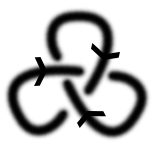
\includegraphics[width=5cm]{inudos/3fcon1.png}}
	\subfigure[B]{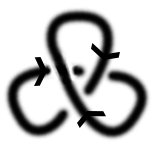
\includegraphics[width=5cm]{inudos/3fcon1neg.png}}
	\subfigure[C]{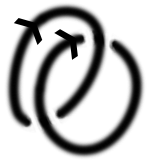
\includegraphics[width=5cm]{inudos/doble1b.png}}
	\caption{Cambio cruces trébol}
	\label{alex2} 
\end{figure}

Al aplicar la segunda regla tendremos:\\
\begin{equation}
\vartriangle(A) - \vartriangle(B) +  (t^{\frac{1}{2}} - t^{\frac{-1}{2}}) \vartriangle(C)  = 0.
\end{equation}
Sabemos que $\vartriangle(B)$ = $\vartriangle$($\bigcirc$)= 1. Luego nos quedaría la ecuación:
\begin{equation}
\vartriangle(A) +  (t^{\frac{1}{2}} - t^{\frac{-1}{2}}) \vartriangle(C)  = 1.
\end{equation}
Ahora necesitamos conocer el valor de $\vartriangle(C)$. Al igual que ocurría anteriormente, la proyección de este nuevo nudo tiene más de un cruce de modo que vamos a aplicarle la segunda regla. Esta vez seleccionamos el cruce superior como cruce que se modifica en los nuevos nudos. Obtenemos las proyecciones que vemos en la figura \ref{alex3}, a las que llamaremos D y E. 
\begin{figure}[h!]
	\centering
	\subfigure[D]{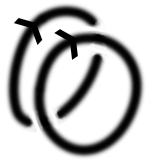
\includegraphics[width=5cm]{inudos/doble2b.png}}
	\subfigure[E]{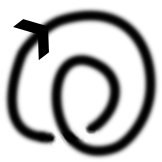
\includegraphics[width=5cm]{inudos/doble3b.png}}
	\caption{Cambio cruces}
	\label{alex3} 
\end{figure}

Al aplicar la segunda regla tendremos:\\
\begin{equation}
\vartriangle(C) - \vartriangle(D) +  (t^{\frac{1}{2}} - t^{\frac{-1}{2}}) \vartriangle(E)  = 0.
\end{equation}

Sabemos que $\vartriangle(E)$ = $\vartriangle$($\bigcirc$)= 1. Además $\vartriangle(D)$ = $\vartriangle$($\bigcirc$ $\bigcirc$)= 0. Luego nos quedaría la ecuación:
\begin{equation}
\vartriangle(C) = -  (t^{\frac{1}{2}} - t^{\frac{-1}{2}}).
\end{equation}

Volviendo a la ecuación (2) tendemos:
\begin{equation}
\vartriangle(A) =  (t^{\frac{1}{2}} - t^{\frac{-1}{2}})^{2} + 1 = t^{-1} -1 + t.
\end{equation}
Luego $ t^{-1} -1 + t $ es el polinomio de Alexander del nudo trébol. \\

\bigskip
Es importante destacar el hecho de que podemos tener un nudo no trivial que tenga como polinomio de Alexander el polinomio trivial equivalente a 1. Por este motivo, con dicho invariante no podemos distinguir cualquier nudo del nudo trivial. \\

¿Mediante estas dos reglas podremos obtener siempre el polinomio de Alexander en tiempo finito? La respuesta es afirmativa, veámoslo:\\

La idea que vamos a seguir en este proceso será reducir las proyecciones, a las que le queremos obtener el polinomio de Alexander, hasta llegar al nudo trivial. Reducir estas proyecciones quiere decir ir modificando sus cruces obteniendo $L_{+}$, $L_{-}$ y $L_{0}$ . Como veíamos en el invariante de la sección \ref{subunk}, a cualquier proyección le podemos aplicar una secuencia finita de cambios en los cruces de modo que resulte el nudo trivial. Por tanto, este procedimiento tendrá fin en una secuencia finita de pasos.\\

Al ir considerando los distintos nudos de la proyección, obtendremos dos nuevas proyecciones en cada paso. Con estas nuevas proyecciones podremos formar lo que se denomina \textbf{ árbol de resolución}. En la figura \ref{alex4} podemos ver el árbol de resolución del nudo trébol.\\

\begin{figure}[h!]
	\centering
	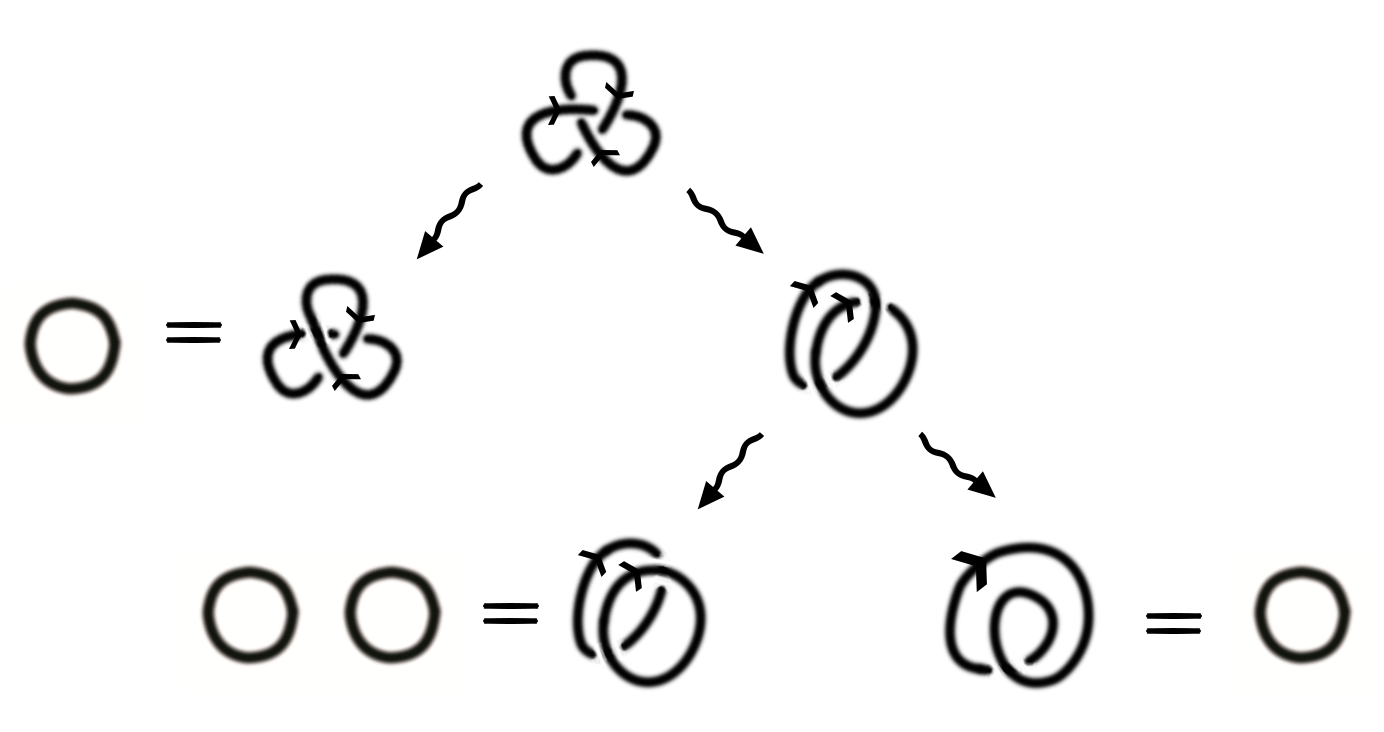
\includegraphics[width=18cm]{inudos/arbol.png}
	\caption{Árbol de resolución del nudo trébol.}
	\label{alex4} 
\end{figure}

\underline{\textbf{Definición:}}\\
Se define la \textbf{profundidad de un nudo} (o enlace) como el mínimo número de niveles que nos encontramos en los árboles de resolución del nudo. \\

Esta profundidad del nudo es un invariante que además nos permite medir la complejidad que supondrá el cálculo del polinomio de Alexander. \\

El árbol de resolución del nudo trébol que vemos en la figura \ref{alex4} tiene una profundidad de 2 niveles (la proyección inicial no se cuenta como nivel). Es importante destacar que el único nudo que tiene profundidad de nudo igual a 0 es el nudo trivial. \\